\documentclass[11pt, oneside]{article}
\usepackage[margin=1in]{geometry}
\geometry{letterpaper}
\usepackage{amssymb}
\usepackage[fleqn]{amsmath}
\usepackage[sharp]{easylist}
\usepackage{relsize}
\usepackage{graphicx}

\pagenumbering{gobble}              % No page numbering
\setlength{\parindent}{0em}         % No paragraph indenting
\setlength{\parskip}{0.5em}         % Paragraph spacing

\newcommand*{\begineasylist}{\begin{easylist}[itemize]\ListProperties(Style*=$\bullet$\quad, Style2*=\tiny$\blacksquare$\quad, Style3*=$\circ$\quad, Style4*=$\diamond$\quad, FinalSpace=1em, Space=0em, Space*=0em)}

\newcommand*{\begineasylistnumbered}{\begin{easylist}[enumerate]\ListProperties(Numbers=a, Space=0em, Space*=0em)}

\newcommand*{\un}[1]{\underline{\smash{#1}}}        % custom underline macro

\begin{document}

\section*{CS 341}

These notes are meant to be supplementary to lecture slides \& the textbook, and so may not contain all covered materials. Here I've chosen content which might not be easy to remember and/or is helpful to look at when doing assignments.

\subsection*{Asymptotic Analysis}
\begineasylist

# \textbf{Order Notations}:
## $f(n) \in O(g(n))$ if $\exists \ c > 0$ and $n_0 > 0$ such that $0 \leq f(n) \leq cg(n) \ \forall \ n \geq n_0$
### $f$ ``grows no faster than'' $g$

## $f(n) \in \Omega(g(n))$ if $\exists \ c > 0$ and $n_0 > 0$ such that $0 \leq cg(n) \leq f(n) \ \forall \ n \geq n_0$
### $f$ ``grows no slower than'' $g$

## $f(n) \in \Theta(g(n))$ if $\exists \ c_1, c_2 > 0$ and $n_0 > 0$ such that $0 \leq c_1g(n) \leq f(n) \leq c_2g(n) \ \forall \ n \geq n_0$
### $f$ ang $g$ have the same complexity

## $f(n) \in o(g(n))$ if $\forall \ c > 0, \exists \ n_0 > 0$ such that $0 \leq f(n) < cg(n) \ \forall \ n \geq n_0$
### $f$ has lower complexity than $g$

## $f(n) \in \omega(g(n))$ if $\forall \ c > 0, \exists \ n_0 > 0$ such that $0 \leq cg(n) < f(n) \ \forall \ n \geq n_0$  
### $f$ has higher complexity than $g$

## $f \in O(g)$ and $f \in \Omega(g) \iff f \in \Theta(g)$

# \textbf{Limit method}: suppose $L = \lim_{n \rightarrow \infty} \dfrac{f(n)}{g(n)}$
## $f \in o(g)$ if $L = 0$
## $f \in \Theta(g)$ if $0 < L < \infty$
## $f \in \omega(g)$ if $L = \infty$

# Useful facts for first-principles proofs:
## $\log n \geq 1 \ \forall \ n \geq 2$; i.e. $\log n$ grows faster than $1$
## $\log n \leq n \ \forall \ n \geq 0$; i.e. $\log n$ grows slower than $n$

# Useful limit laws:
## $\lim_{n\rightarrow\infty} \dfrac{f(n)}{g(n)} = \lim_{n\rightarrow\infty} \dfrac{\log(f(n))}{\log(g(n))}$
## $\lim_{n\rightarrow\infty} f(n)^k = (\lim_{n\rightarrow\infty} f(n))^k$

# Some math rules:
## Summing a polynomial: $\sum_{i=1}^n i^k \in \Theta(n^{k+1})$
## Summing an exponential (special case of geometric series):
$$\sum_{i=1}^n c^i \in \left\{
\begin{array}{ll}
\Theta(c^{n+1}) &\text{if } c > 1 \\
\Theta(n) &\text{if } c = 1 \\
\Theta(1) &\text{if } c < 1
\end{array}
\right.
$$
## $a^{\log_b n} = n^{\log_b a}$ (Useful for recursion trees)
## Geometric series:
$$\sum_{i=0}^{n-1}ar^i = \left\{
\begin{array}{ll}
a\frac{r^n-1}{r-1} \in \Theta(r^n) &\text{if } r > 1 \\
na \in \Theta(n) &\text{if } r = 1 \\
a\frac{1-r^n}{1-r} \in \Theta(1) &\text{if } r < 1
\end{array}
\right.
$$
## $a \geq b + c$ if $a \geq 2 \cdot \max(b, c)$ (useful for asymtotic proofs)
## $\lim_{x \rightarrow c} \dfrac{f(x)}{g(x)} = \lim_{x \rightarrow c} \dfrac{f'(x)}{g'(x)}$ if it exists (L'Hopital's Rule)
## $\log (n!) \in \Theta(n \log n)$ (Stirling's Approximation)
## $\sum_{i=1}^n \dfrac{1}{i} \in \Theta(\log n)$ (Harmonic series)

\end{easylist}
\newpage
\subsection*{Divide and Conquer}
\begineasylist

# \textbf{Recursion-tree method}:
## Given the recurrence $T(n) = aT(n/b) + f(n), T(1) = c$:
### $a$ is the \# of recursive calls made (\# of subproblems) 
### $b$ is the \# by which the input size $n$ is divided in each recursive call
### $f(n)$ is the runtime of the ``work done outside of the recursive calls''
### $c$ is the constant-time work done in each recursive call in the base case
## Each node of the recursion tree represents the cost of the work done other than making recursive calls
## Each row represents the total cost of work done in all recursive calls at that recursion ``level'' 
## The height of the tree depends on the factor that the input size is divided by; i.e. $\log_b n$
## E.g.: Picture this as a tree where each node (except for leaves) has $a$ children;
\begin{align*}
&\text{Level 0:} \qquad f(n) &&\text{total} = f(n)\\
&\text{Level 1:} \qquad f(n/b) \qquad \ldots \qquad f(n/b) &&\text{total} = af(n/b) \\
&\text{Level 2:} \qquad f(n/b^2) \qquad \ldots \qquad f(n/b^2) &&\text{total} = a^2f(n/b^2) \\
&\ldots \\
&\text{Level $k$:} \qquad f(n/b^k) \qquad \ldots \qquad f(n/b^k) &&\text{total} = a^kf(n/b^k) \\
&\ldots \\
&\text{Level $\log_b n$:} \qquad c \qquad \ldots \qquad c &&\text{total} = ca^{\log_b n} = cn^{\log_b a}
\end{align*}
### Total runtime of recursion tree is (summing every row total):
$$T(n) \in \Theta\left(\sum_{i=0}^{\log_b n - 1} a^if(n/b^i)\right) + \Theta(n^{\log_b a})$$
### Use geometric series formula to find a simplified value

\newpage
## Example: $T(n) = 3T(n/4) + n^2$ \\
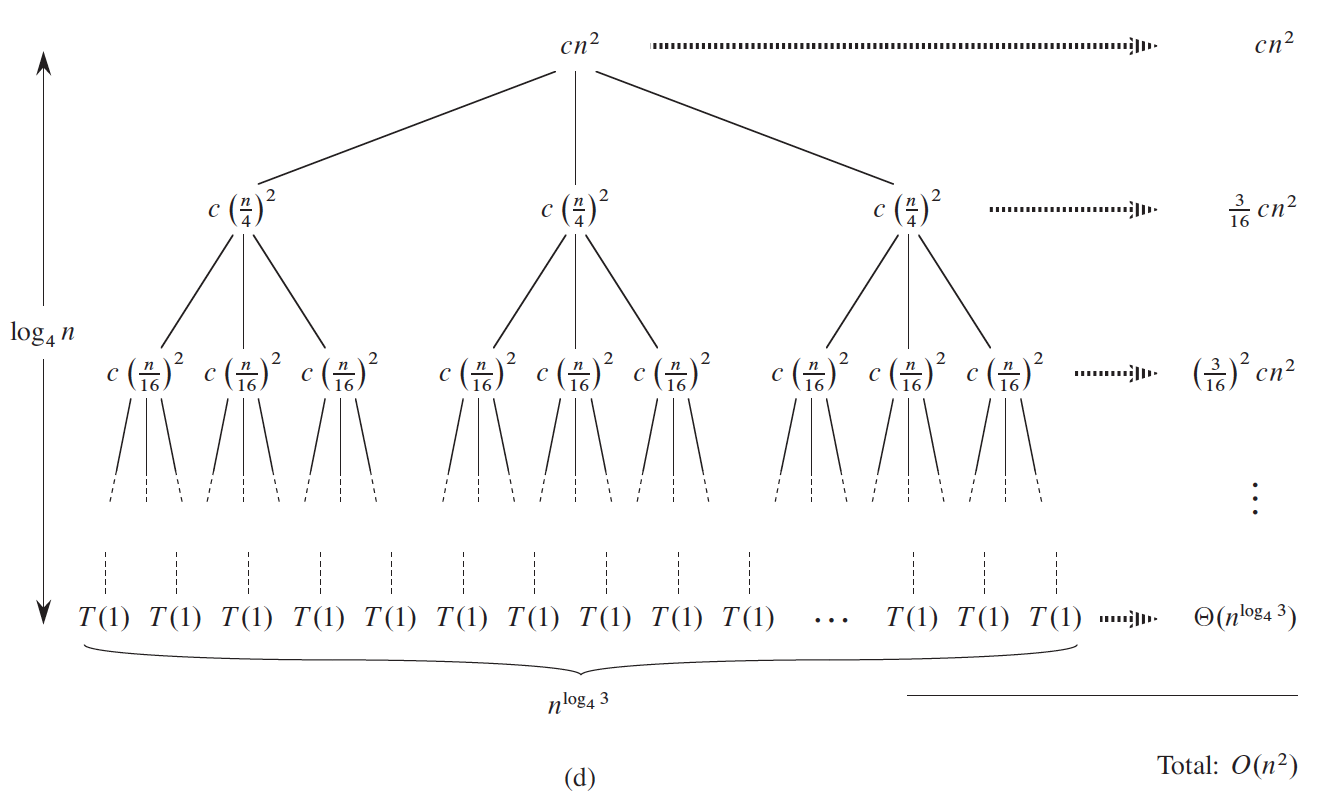
\includegraphics[width=0.8\textwidth]{rec_tree.png}
$$T(n) \in \Theta\left(\sum_{k=0}^{\log_4 n - 1} \left(\frac{3}{16}\right)^k n^2 + n^{\log_4 3}\right) \in \Theta(n^2)$$

# \textbf{Master method}:
## Given the recurrence $T(n) = aT(n/b) + f(n)$ where $f(n) \in \Theta(n^d)$:
$$T(n) \in \left\{
\begin{array}{ll}
\Theta(n^{\log_b a}) &\text{if } a > b^d \\
\Theta(n^d\log n) &\text{if } a = b^d \\
\Theta(n^d) &\text{if } a < b^d
\end{array}
\right.
$$


\end{easylist}
\newpage
\subsection*{Greedy Algorithms}
\begineasylist

# Two methods of proving greedy algorithms:

# \textbf{Greedy stays ahead (induction)}
## Show that $S_g$ is better than $S$ at every step
## \un{Base case}: show $S_g[1] > S[1]$
## \un{Inductive hypothesis}: assume $S_g[k-1] > S[k-1]$; show that $S_g[k] > S[k]$
### Often by contradiction; i.e. suppose $\exists \ S^*$ such that $S_g[k] < S^*[k]$, and derive some contradiction

# \textbf{Exchange argument (swapping)}
## Let $S_g$ = greedy solution, $S$ = some arbitrary solution
## Show that (any) $S$ can be transformed into $S_g$ step-by-step \un{without getting worse at any point}
### i.e. compare the cost of before \& after swapping 2 elements in $S$, show that it doesn't change or improves



\end{easylist}
\newpage
\subsection*{Intractability}
\begineasylist

# $P$: \un{solvable} in \un{polynomial time}
# $NP$: \un{verifiable} in \un{polynomial time}
## $P \subseteq NP$
# $NP$-complete: set of problems $X \in NP$ such that all $Y \in NP$ can be reduced to $X$
## $NPC \subseteq NP$


# \textbf{Reducibility}:
## $L_1 \leq_P L_2$ -- ``$L_1$ is polynomial-time reducible to $L_2$''
## There exists a P-time computable function that maps $L_1$ to $L_2$ \\
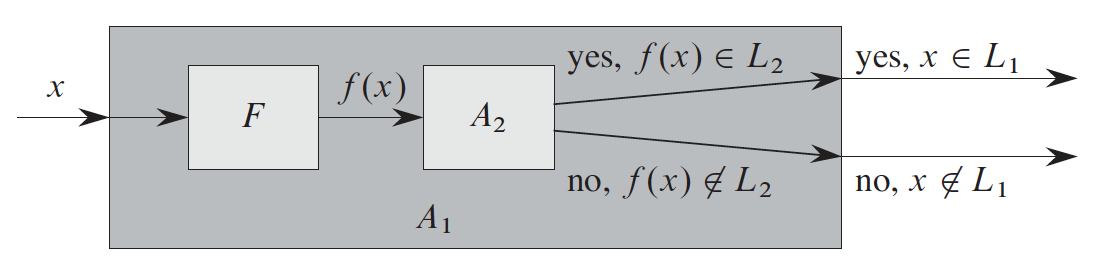
\includegraphics[width=0.6\textwidth]{reduction.png}

## If $L_1 \leq_P L_2$, then $L_2 \in P \implies L_1 \in P$
### i.e., if $L_2$ is solvable in P-time, then $L_1$ is as well
### i.e., $L_1$ is \un{no harder than} $L_2$ 

## Contrapositive:
### i.e., if $L_1$ is known to be \emph{not} solvable in P-time, then $L_2$ can't be either
### i.e. $L_2$ is \un{as hard as} $L_1$


\end{easylist}
\end{document}